\documentclass[12pt]{article}
\usepackage[utf8]{inputenc}
\usepackage{float}
\usepackage{amsmath}
\usepackage{amssymb}
\usepackage{tkz-euclide}


\usepackage[hmargin=3cm,vmargin=6.0cm]{geometry}
%\topmargin=0cm
\topmargin=-2cm
\addtolength{\textheight}{6.5cm}
\addtolength{\textwidth}{2.0cm}
%\setlength{\leftmargin}{-5cm}
\setlength{\oddsidemargin}{0.0cm}
\setlength{\evensidemargin}{0.0cm}

%misc libraries goes here

\newcommand{\Z}{\mathbb{Z}}
\newcommand{\R}{\mathbb{R}}

\begin{document}

\section*{Student Information } 
%Write your full name and id number between the colon and newline
%Put one empty space character after colon and before newline
Full Name : Onat Özdemir \\
Id Number : 2310399 \\

% Write your answers below the section tags
\section*{Answer 1}
\renewcommand{\theenumi}{\alph{enumi}}
\begin{enumerate}
\item Let $a$ be the number of all bit strings of length 9 which satisfy the given condition and $A_{n}$ be a set that contains all possible binary strings of length 9 which satisfy the given condition and contains n 1's. Since each 1 followed by 0, then $2n < 9$. Hence, the maximum number of 1's that can be stored in the binary string of 9 is 4. Each $A_{n}$ where $n \in \{1,2,3,4\}$ pairwise disjoint since each $A_{n}$ differs from others with the number of 1s it contains, then by the rule of sum,
\begin{equation}
\begin{split}
a = |A_{1}| + |A_{2}| + |A_{3}| + |A_{4}|
\end{split}
\end{equation}
Since, by the given rule, each 1 must  exists with a 0 placed in the right side of the 1, for the rest of the question each "10" string fragment will be represented by "x" symbol.\\
Then, in order to find a, let us find the values of $|A_{1}|,\ |A_{2}|,\ |A_{3}| $ and $|A_{4}|$.\\ \\
For n = 1, each bit strings of length 9 which satisfy the given condition will be the one of the permutations of 1 x and 7 0's. So, by using permutation with indistinguishable objects rule,
\begin{equation}
\begin{split}
|A_{1}| = \frac{8!}{7!*1!} = 8
\end{split}
\end{equation}
For n = 2, each bit strings of length 9 which satisfy the given condition will be the one of the permutations of 2 x's and 5 0's. So, by using permutation with indistinguishable objects rule,
\begin{equation}
\begin{split}
|A_{2}| = \frac{7!}{5!*2!} = 21
\end{split}
\end{equation}
For n = 3, each bit strings of length 9 which satisfy the given condition will be the one of the permutations of 3 x's and 3 0's. So, by using permutation with indistinguishable objects rule,
\begin{equation}
\begin{split}
|A_{3}| = \frac{6!}{3!*3!} = 20
\end{split}
\end{equation}
For n = 4, each bit strings of length 9 which satisfy the given condition will be the one of the permutations of 4 x's and 1 0. So, by using permutation with indistinguishable objects rule,
\begin{equation}
\begin{split}
|A_{4}| = \frac{5!}{4!*1!} = 5
\end{split}
\end{equation}
Hence, by using (1),(2),(3),(4) and (5),
\begin{equation*}
\begin{split}
a = 8 + 21 + 20 + 5 = 54
\end{split}
\end{equation*}

\item Let $S$ be the set of all bit strings of length 10 which have at least eight 1s and $A_{i}$ be the set of all bit strings of length 10 which contain i 1's. Then,
\begin{equation*}
\begin{split}
S = \bigcup\nolimits_{i = 8}^{10} A_{i}
\end{split}
\end{equation*}
Since each $A_{i}$ differs from each other with number of 1's it contains, we can conclude that each $A_{i}$ is pairwise disjoint. Then, by the rule of sum,
\begin{equation}
\begin{split}
|S| = \sum_{i=8}^{10} |A_{i}|
\end{split}
\end{equation}
Then, let us find $|A_{8}|,\ |A_{9}|$ and $|A_{10}|$. \\
For i = 8, each bit strings of length 10 will be the one of the permutations of 8 1's and 2 0's. So, by using permutation with indistinguishable objects rule,
\begin{equation}
\begin{split}
|A_{8}| = \frac{10!}{8!*2!} = 45
\end{split}
\end{equation}
For i = 9, each bit strings of length 10 will be the one of the permutations of 9 1's and 1 0. So, by using permutation with indistinguishable objects rule,
\begin{equation}
\begin{split}
|A_{9}| = \frac{10!}{9!*1!} = 10
\end{split}
\end{equation}
For i = 10, each bit strings of length 10 will be the one of the permutations of 10 1's. So, by using permutation with indistinguishable objects rule,
\begin{equation}
\begin{split}
|A_{10}| = \frac{10!}{10!*1} = 1
\end{split}
\end{equation}
Hence, by using (6), (7), (8) and (9),
\begin{equation}
\begin{split}
|S| = 45 + 10 + 1 = 56
\end{split}
\end{equation}


\item Let our set with 4 elements be $S = \{x_{1},x_{2},x_{3},x_{4}\}$.\\
 By the definition, an onto function from set S with 4 elements to set B with 3 elements denotes that every element in B is an image of some element in S which implies that there is a partition of S with 3 subsets such that each subset has a unique image in B. So that, the number of possible onto functions from S to B equals to the number of possible one to one functions from these partition set to B.
 
 Then, let us find all possible partitions of S with 3 subsets,
 \begin{equation*}
 \begin{split}
 P_{1} = \{\{x_{1}\},\{x_{2}\},\{x_{3},x_{4}\}\} & \\
 P_{2} = \{\{x_{1}\},\{x_{3}\},\{x_{2},x_{4}\}\}& \\
 P_{3} = \{\{x_{2}\},\{x_{3}\},\{x_{1},x_{4}\}\}& \\
 P_{4} = \{\{x_{4}\},\{x_{2}\},\{x_{1},x_{3}\}\}& \\
 P_{5} = \{\{x_{4}\},\{x_{3}\},\{x_{1},x_{2}\}\}& \\
 P_{6} = \{\{x_{4}\},\{x_{1}\},\{x_{2},x_{3}\}\}
 \end{split}
 \end{equation*}
 Hence, the number of all possible partitions of S with 3 subsets is 6.\\
 Since number of elements that B contains is 3, the number of all possible one to one functions from the $P_{i}$ where $i\in\{1,2,3,4,5,6\}$ to B is 3! = 3.2.1 = 6. Then, by the multiplication rule, the number of all possible onto functions from S to B is,
 \begin{equation*}
 \begin{split}
 6*3!  = 6*6 = 36
 \end{split}
 \end{equation*}



\item The capacity of our collection is 4. However, since at least one Discrete Mathematics textbook and at least one Signals and Systems textbook must
be in the collection, we need to select 2 books for the remaining 2 place. Since the order in the collection is not important, we should use combination. Moreover, since the repetition is allowed, we can use the formula of the combination with repetition placed in the Rosen's Book page 425, \\
\begin{equation}
\begin{split}
C(n+r-1,r) 
\end{split}
\end{equation}
where $n$ represents the number of book types and $r$ represents the number of book we need to choose. For our case since we have two types of book, $n = 2$ and since we need to choose 2 books, $r=2$. Then, place these numbers to (11),
\begin{equation}
\begin{split}
C(2+2-1,2) = C(3,2) = \frac{3!}{2!1!} = 3
\end{split}
\end{equation}
Thus, from (12), we can make the collection with the given properties from the given books in 3 different ways.
\end{enumerate}

\section*{Answer 2}
\renewcommand{\theenumi}{\alph{enumi}}
\begin{enumerate}
\item 
Firstly, let us find $a_{1}$ and $a_{2}$, since they will be our initial conditions.For n = 1, given set will be \{1\}. So, the set that contains the subsets of the given set will be $\{\emptyset, \{1\}\}$. Since both elements of this set satisfies the initial condition, $a_{1} = 2$. For n = 2, given set will be $\{1,2\}$. So, the set that contains the subsets of the given set will be $\{\emptyset, \{1\}, \{2\}, \{1,2\} \}$.Since every element except $\{1,2\}$ of this set satisfies the initial condition, $a_{2} = 3$.
\\ \\
Let $S_{n}$ be a set contains the all subsets of the set \{1, 2, 3 ... n\} that does not contain two consecutive numbers.
Let $S_{n}^{(0)}$ = $\{A \ | \ A\in S_{n}\land n\notin A\}$ and $S_{n}^{(1)}$ = $\{A \ | \ A\in S_{n}\land n\in A\}$. Since $S_{n}^{(0)}\cap S_{n}^{(1)} = \emptyset$ and $S_{n}^{(0)}\cup S_{n}^{(1)} = S_{n}$, by the rule of sum,
\begin{equation}
\begin{split}
|S_{n}| = a_{n} = |S_{n}^{(0)}|+|S_{n}^{(1)}|
\end{split}
\end{equation}
Then, let us find $|S_{n}^{(1)}|$ for $n \geq 3$. To satisfy the definition of $S_{n}^{(1)}$, we can say that for an arbitrarily chosen $A\in S_{n}^{(1)}$, $(n-1)\notin A$ must also satisfy. Then, by the definition we made,
\begin{equation}
\begin{split}
S_{n}^{(1)} = \{A \cup \{n\} \ | \ A\in S_{n-2} \}
\end{split}
\end{equation}
Hence, 
\begin{equation}
\begin{split}
|S_{n}^{(1)}| = |S_{n-2}| = a_{n-2}
\end{split}
\end{equation}
Let us find $|S_{n}^{(0)}|$ for $n \geq 3$.
By the definition we made, it can be easily seen that $S_{n}^{(0)} = S_{n-1} = \{A \ | \ A\in S_{n}\land n\notin A\}$. Hence, 
\begin{equation}
\begin{split}
|S_{n}^{(0)}| = |S_{n-1}| = a_{n-1}
\end{split}
\end{equation}
Then, by using (13), (15) and (16), 
\begin{equation}
\begin{split}
|S_{n}| = a_{n} = a_{n-1} + a_{n-2} \qquad  for \ n \geq 3 \qquad a_{1}=2,\ a_{2}=3
\end{split}
\end{equation}



\item First note that, although $a_{0}$ is not a suitable case for this problem, in order to maintain the power series concept we can find it's value from (17),
\begin{equation*}
\begin{split}
a_{2} = a_{1} + a_{0} \qquad & \\ 
3 = 2 + a_{0} \qquad
\end{split}
\end{equation*}
From now on, we will use $a_{0}$ with value 1.

Let's define a generating function $G(x)$ such that,
\begin{equation}
\begin{split}
G(x) = \sum_{n=0}^{\infty} a_{n}x^{n} 
\end{split}
\end{equation}
Then,
\begin{equation}
\begin{split}
\sum_{n=2}^{\infty} a_{n}x^{n} = G(x)-a_{0}-a_{1}x = G(x) -1 -2x 
\end{split}
\end{equation}
Also,
\begin{equation}
\begin{split}
\sum_{n=1}^{\infty} a_{n-1}x^{n} = xG(x) 
\end{split}
\end{equation}
Rearrange (20),
\begin{equation}
\begin{split}
\sum_{n=2}^{\infty} a_{n-1}x^{n} = xG(x)-a_{0}x = xG(x)-x 
\end{split}
\end{equation}
Moreover,
\begin{equation}
\begin{split}
\sum_{n=2}^{\infty} a_{n-2}x^{n} = x^2G(x) 
\end{split}
\end{equation}
Then, since the starting values of (19), (21) and (22) are same,
\begin{equation}
\begin{split}
\sum_{n=2}^{\infty} a_{n}x^{n}-\sum_{n=2}^{\infty} a_{n-1}x^{n}-\sum_{n=2}^{\infty} a_{n-2}x^{n} = \sum_{n=2}^{\infty} (a_{n}-a_{n-1}-a_{n-2})x^{n}
\end{split}
\end{equation}
From (19), (21), (22) and (23)
\begin{equation}
\begin{split}
\sum_{n=2}^{\infty} (a_{n}-a_{n-1}-a_{n-2})x^{n} =  G(x) -1 -2x-xG(x)+x -x^2G(x)
\end{split}
\end{equation}
From (17),
\begin{equation*}
\begin{split}
a_{n}-a_{n-1}-a_{n-2} = 0
\end{split}
\end{equation*}
Then,
\begin{equation}
\begin{split}
\sum_{n=2}^{\infty} (a_{n}-a_{n-1}-a_{n-2})x^{n} = 0 = G(x) -1 -2x-xG(x)+x -x^2G(x)
\end{split}
\end{equation}
Rearrange (25),
\begin{equation}
\begin{split}
G(x)= \frac{1+x}{1-x-x^2}
\end{split}
\end{equation}
Apply partial fractions method to (26),
\begin{equation}
\begin{split}
G(x) = \frac{\frac{10+6\sqrt{5}}{20}}{1-\frac{1+\sqrt{5}}{2}x} + \frac{\frac{10-6\sqrt{5}}{20}}{1-\frac{1-\sqrt{5}}{2}x}
\end{split}
\end{equation}
Since, 
\begin{equation*}
\begin{split}
\frac{1}{1-kx} = \sum_{n=0}^{\infty}{(kx)^n}
\end{split}
\end{equation*}
Then, we can represent (27) as,
\begin{equation*}
\begin{split}
G(x) = \sum_{n=0}^{\infty}{((\frac{10+6\sqrt{5}}{20})(\frac{1+\sqrt{5}}{2})^n+(\frac{10-6\sqrt{5}}{20})(\frac{1-\sqrt{5}}{2})^n)*x^n}
\end{split}
\end{equation*}
Then from (18),
\begin{equation*}
\begin{split}
\sum_{n=0}^{\infty} a_{n}x^{n} = \sum_{n=0}^{\infty}{((\frac{10+6\sqrt{5}}{20})(\frac{1+\sqrt{5}}{2})^n+(\frac{10-6\sqrt{5}}{20})(\frac{1-\sqrt{5}}{2})^n)*x^n}
\end{split}
\end{equation*}
Thus,
\begin{equation*}
\begin{split}
a_{n} = (\frac{10+6\sqrt{5}}{20})(\frac{1+\sqrt{5}}{2})^n+(\frac{10-6\sqrt{5}}{20})(\frac{1-\sqrt{5}}{2})^n \qquad n \geq 1
\end{split}
\end{equation*}


\end{enumerate}

\section*{Answer 3}
Since the given recurrence relation is linear homogeneous recurrence relation with constant coefficients, we can benefit from the characteristic equation of it in order to find the solution;\\ \\
Rearrange the given relation,
\begin{equation}
\begin{split}
a_{n} -4a_{n-1} - a_{n-2} + 4a_{n-3} = 0
\end{split}
\end{equation}
So characteristic equation of (28) will be,
\begin{equation}
\begin{split}
r^3 - 4r^2 -r + 4 = 0
\end{split}
\end{equation}
If we rearrange (29),
\begin{equation}
\begin{split}
r^3 - 4r^2 -r + 4 = (r+1)(r-1)(r-4) = 0
\end{split}
\end{equation}
Then, the characteristic roots of (30),
\begin{equation}
\begin{split}
r_{1} = -1, \qquad r_{2} = 1, \qquad r_{3} = 4
\end{split}
\end{equation}
As can be seen from (31),
\begin{equation}
\begin{split}
r_{1} \neq  r_{2} \neq r_{3}
\end{split}
\end{equation}
Hence, multiplicity of each characteristic root is 1. Therefore, we can claim that the solution of $a_{n}$ will be in the form,\\
\begin{equation}
\begin{split}
a_{n} = \alpha_{1}.(-1)^n + \alpha_{2}.(1)^n + \alpha_{3}.(4)^n \qquad \alpha_{1},\alpha_{2},\alpha_{3} \in \R
\end{split}
\end{equation}
To find the constants $\alpha_{1},\alpha_{2},\alpha_{3}$, we can use the initial conditions,
\begin{equation}
\begin{split}
a_{0} = \alpha_{1}.(-1)^0 + \alpha_{2}.(1)^0 + \alpha_{3}.(4)^0 = \alpha_{1} + \alpha_{2} + \alpha_{3} = 4 & \\ a_{1} = \alpha_{1}.(-1)^1 + \alpha_{2}.(1)^1 + \alpha_{3}.(4)^1 = -\alpha_{1} + \alpha_{2} + 4\alpha_{3} = 8 & \\ a_{2} = \alpha_{1}.(-1)^2 + \alpha_{2}.(1)^2 + \alpha_{3}.(4)^2 = \alpha_{1} + \alpha_{2} + 16\alpha_{3} = 34
\end{split}
\end{equation}
When these three simultaneous equations are solved for $\alpha_{1},\alpha_{2},\alpha_{3}$,
\begin{equation}
\begin{split}
\alpha_{1} =1,\qquad \alpha_{2} =1, \qquad \alpha_{3} = 2
\end{split}
\end{equation}
Hence, from (33) and (35), the solution of given recurrence relation with given initial conditions is,
\begin{equation*}
\begin{split}
a_{n} = 1.(-1)^n + 1.(1)^n + 2.(4)^n \qquad n \geq 0
\end{split}
\end{equation*}


\section*{Answer 4}
By the definition of equivalence relations, in order to prove R is an equivalence relation, we need to prove R is a reflexive, symmetric and transitive relation.\\
\textbf{Proof of R is Reflexive:}
In order to prove R is a reflexive relation, we have to prove that $\forall x,y\in \R((x,y)R(x,y))$. Let's choose arbitrary $x$ and $y$ such that $x,y \in \R$.Then, assume that,
\begin{equation}
\begin{split}
3x-2y \neq 3x-2y
\end{split}
\end{equation}
 If we rearrange (36), we obtain,
 \begin{equation}
 \begin{split}
 0 \neq 0
 \end{split}
 \end{equation}
 Since, (37) is false, by using proof by contradiction, we can conclude,
 \begin{equation}
 \begin{split}
 3x-2y = 3x-2y
 \end{split}
 \end{equation}
 Then, since (38) satisfies the given property of R, we can conclude that,
 \begin{equation}
 \begin{split}
 (x,y)R(x,y)
 \end{split}
 \end{equation}
 Moreover, since $x,y \in \R$ are arbitrarily chosen, 
\begin{equation}
\begin{split}
\forall x,y\in \R  \qquad (x,y)R(x,y) \quad 
\end{split}
\end{equation}
Thus, by the definition, we have proved that R is a reflexive relation.\\
\textbf{Proof of R is Symmetric:}
In order to prove R is a symmetric relation, we have to prove that $\forall x_{1},y_{1},x_{2},y_{2}\in \R ((x_{1},y_{1})R(x_{2},y_{2}) \rightarrow (x_{2},y_{2})R(x_{1},y_{1}))$. Let's choose arbitrary $ x_{1},y_{1},x_{2},y_{2}\in \R$ such that $(x_{1},y_{1})R(x_{2},y_{2})$. Then, by the definition of R,
\begin{equation}
\begin{split}
3x_{1}-2y_{1} = 3x_{2}-2y_{2}\quad
\end{split}
\end{equation}
Since $3x_{2}-2y_{2}=3x_{1}-2y_{1}$ holds from (41) by using the symmetry property of equality, then by the given property of R this result implies that $(x_{2},y_{2})R(x_{1},y_{1})$. Moreover, since $ x_{1},y_{1},x_{2},y_{2}\in \R$ are chosen arbitrarily we can conclude that,
\begin{equation}
\begin{split}
\forall x_{1},y_{1},x_{2},y_{2}\in \R ((x_{1},y_{1})R(x_{2},y_{2}) \rightarrow (x_{2},y_{2})R(x_{1},y_{1}))
\end{split}
\end{equation}
Thus, from (42), we have proved that R is a symmetric relation.\\
\textbf{Proof of R is Transitive:}
In order to prove R is a transitive relation, we have to prove that $\forall x_{1},y_{1},x_{2},y_{2},x_{3},y_{3}\in \R((x_{1},y_{1})R(x_{2},y_{2})\land(x_{2},y_{2})R(x_{3},y_{3})\rightarrow (x_{1},y_{1})R(x_{3},y_{3}))$. Let's choose arbitrary $ x_{1},y_{1},x_{2},y_{2},x_{3},y_{3}\in \R$ such that $(x_{1},y_{1})R(x_{2},y_{2})\land(x_{2},y_{2})R(x_{3},y_{3})$ be true. Then by the given property of R,
\begin{equation}
\begin{split}
3x_{1} -2y_{1} = 3x_{2} - 2y_{2}
\end{split}
\end{equation}
and,
\begin{equation}
\begin{split}
3x_{2} -2y_{2} = 3x_{3} - 2y_{3}
\end{split}
\end{equation}
holds. By adding (43) and (44), we can obtain,
\begin{equation}
\begin{split}
3x_{1} -2y_{1} = 3x_{3} - 2y_{3}
\end{split}
\end{equation}
Since (45) satisfies the given property of R, we can conclude that $(x_{1},y_{1})R(x_{3},y_{3})$. Hence, we have proved that $(x_{1},y_{1})R(x_{2},y_{2})\land(x_{2},y_{2})R(x_{3},y_{3})\rightarrow (x_{1},y_{1})R(x_{3},y_{3})$ is true. Moreover, since $ x_{1},y_{1},x_{2},y_{2},x_{3},y_{3}\in \R$ arbitrarily chosen we can conclude that,
\begin{equation}
\begin{split}
\forall x_{1},y_{1},x_{2},y_{2},x_{3},y_{3}\in \R((x_{1},y_{1})R(x_{2},y_{2})\land(x_{2},y_{2})R(x_{3},y_{3})\rightarrow (x_{1},y_{1})R(x_{3},y_{3}))
\end{split}
\end{equation}
Thus, from (46), by the definition, we have proved that R is a transitive relation.\\ \\
We are able to prove that R is a reflexive, symmetric and transitive relation. Thus, by the definition, we have proved that R is an equivalence relation.\\ \\
Since, we have found that R is an equivalence relation then we can find [(2,3)] and [(2,-3)].\\
\textbf{For [(2,3)]}: Let's choose arbitrary $x,y \in \R$ such that $(2,3)R(x,y)$ then by the given property of R,
\begin{equation}
\begin{split}
3*2 -2*3 = 3x - 2y & \\
y = \frac{3x}{2}  \qquad
\end{split}
\end{equation}
Then, the solution set of (47) will be the equivalence class of (2,3). As can be seen, representation of the solution set in the Cartesian Plot, will be in the form of a line whose equation is $y = \frac{3x}{2}$.\\
\textbf{For [(2,-3)]}: Let's choose arbitrary $x,y \in \R$ such that $(2,3)R(x,y)$ then by the given property of R,
\begin{equation}
\begin{split}
3*2 -2*(-3) = 3x - 2y & \\
y = \frac{3x}{2}-6  \qquad
\end{split}
\end{equation}
Then, the solution set of (48) will be the equivalence class of (2,-3). As can be seen, representation of the solution set in the Cartesian Plot, will be in the form of a line whose equation is $y = \frac{3x}{2}-6$.

\begin{figure}[h]
	\centering
	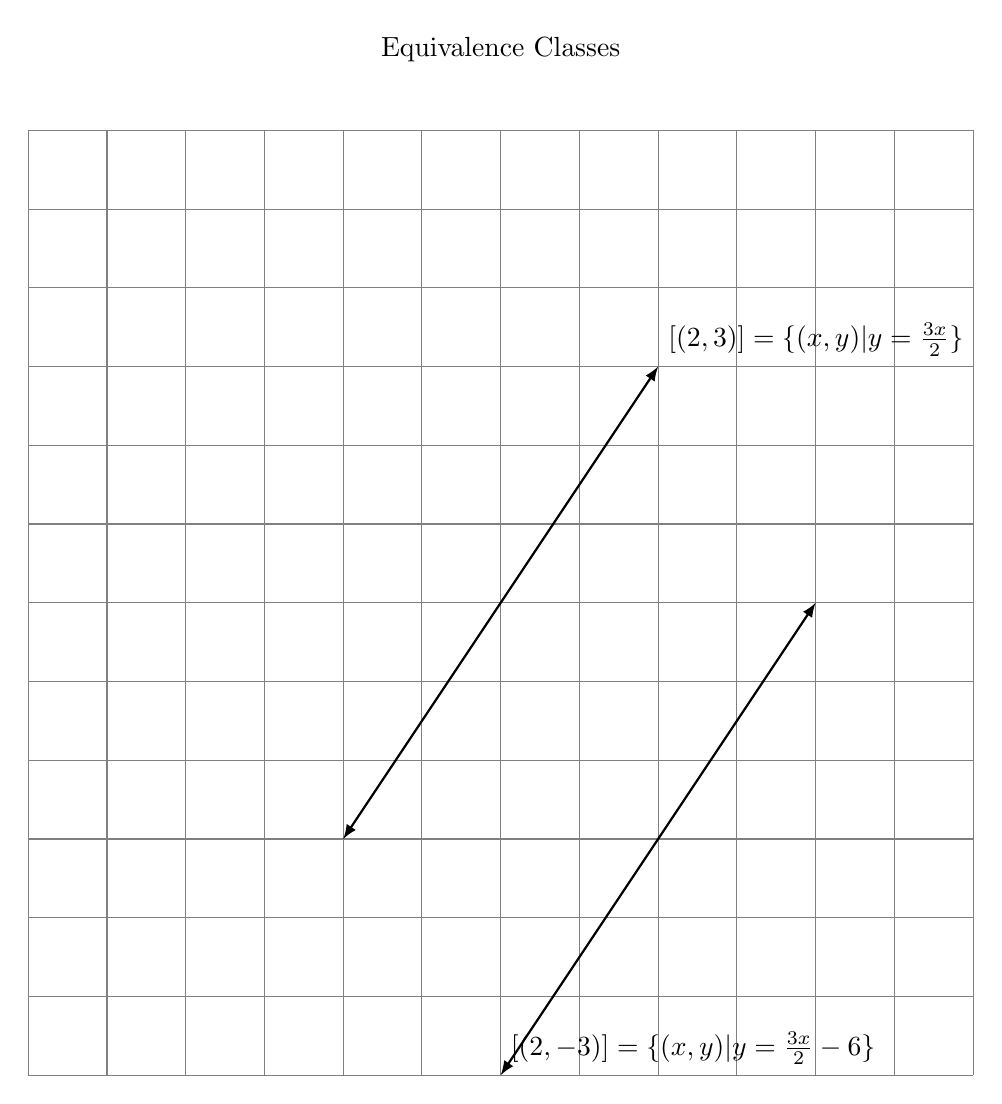
\begin{tikzpicture}
	\tkzInit[xmax=6,ymax=6,xmin=-6,ymin=-6]
	\tkzGrid
	\tkzAxeXY
	\draw[ thick,latex-latex] (-2,-3) -- (2,3) node[anchor=south west] {$[(2,3)] = \{(x,y)|y = \frac{3x}{2}\}$}; % two points for drawing y = 3x/2
	\draw[ thick,latex-latex] (4,0) -- (0,-6) node[anchor=south west] {$[(2,-3)] = \{(x,y)|y =  \frac{3x}{2}-6\}$}; % two points for drawing y = 3x/2
	\tkzText[above](0,6.75){Equivalence Classes}
	\end{tikzpicture}
\end{figure}




\end{document}